\section{Fast Direct Solvers}

\begin{frame}
    \frametitle{FMM-LU: A fast direct solver for BIEs}
    Introduce motivation behind FMM-LU (RS-S).
\end{frame}


\begin{frame}
    \frametitle{Proxy Compression I}
\end{frame}

\begin{frame}

    \frametitle{Proxy Compression II}

\end{frame}

\begin{frame}

    \frametitle{Helmholtz - Sound Hard I}

    \begin{columns}
        \begin{column}{0.5\textwidth}

            Let's consider the exterior acoustic scattering problem in 3D, with sound-hard
            boundary conditions, for low-frequencies.

            \hspace*{0.5pt}

            \centering
            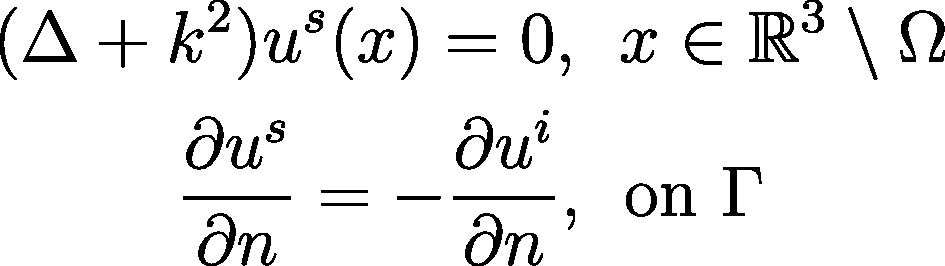
\includegraphics[width=\textwidth]{assets/sound_hard_1.pdf}

        \end{column}

        \begin{column}{0.5\textwidth}
            \begin{center}
                \begin{figure}
                    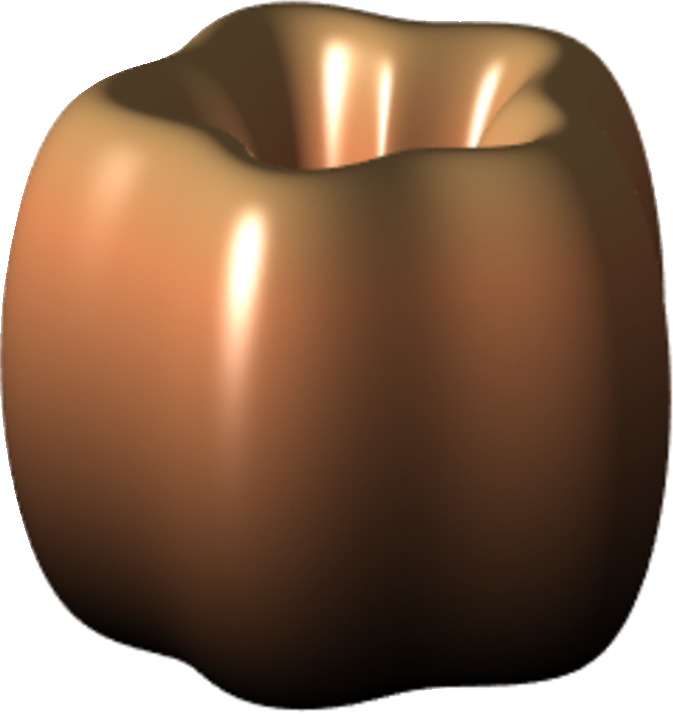
\includegraphics[width=0.6\textwidth]{assets/wiggly_torus.pdf}
                    \caption{`Wiggly Torus', test geometry}
                \end{figure}
            \end{center}
        \end{column}
\end{columns}

\end{frame}

\begin{frame}
    \frametitle{Helmholtz - Sound Hard II}

    Using a regularised representation, form a boundary integral equation.

    \hspace*{0.5pt}

    \centering
    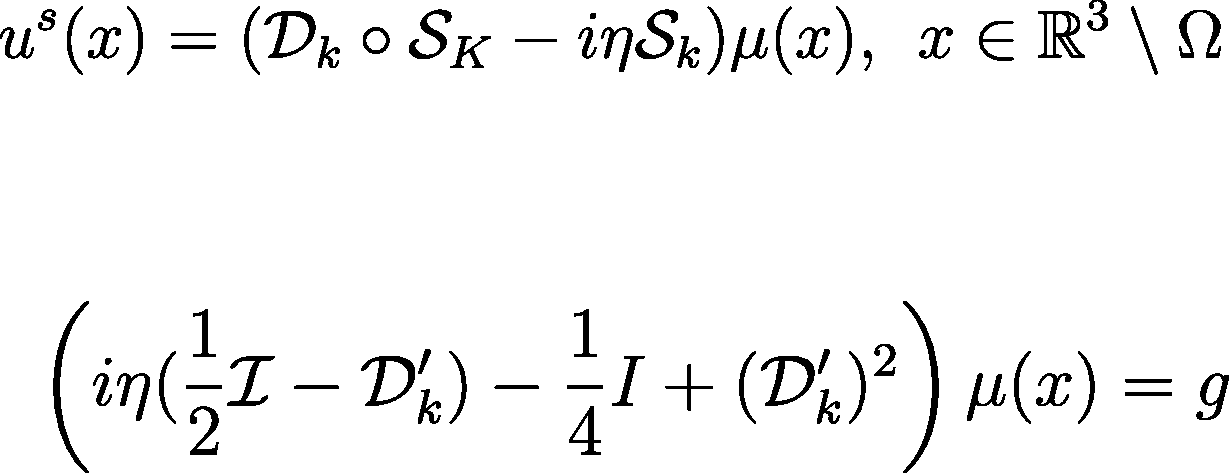
\includegraphics[width=0.6\textwidth]{assets/sound_hard_2.pdf}

\end{frame}

\begin{frame}
    \frametitle{Helmholtz - Sound Hard III}

    Using a Calderon Identity, can form a system of equations, which we proceed
    to discretise.

    \hspace*{0.5pt}

    \centering

    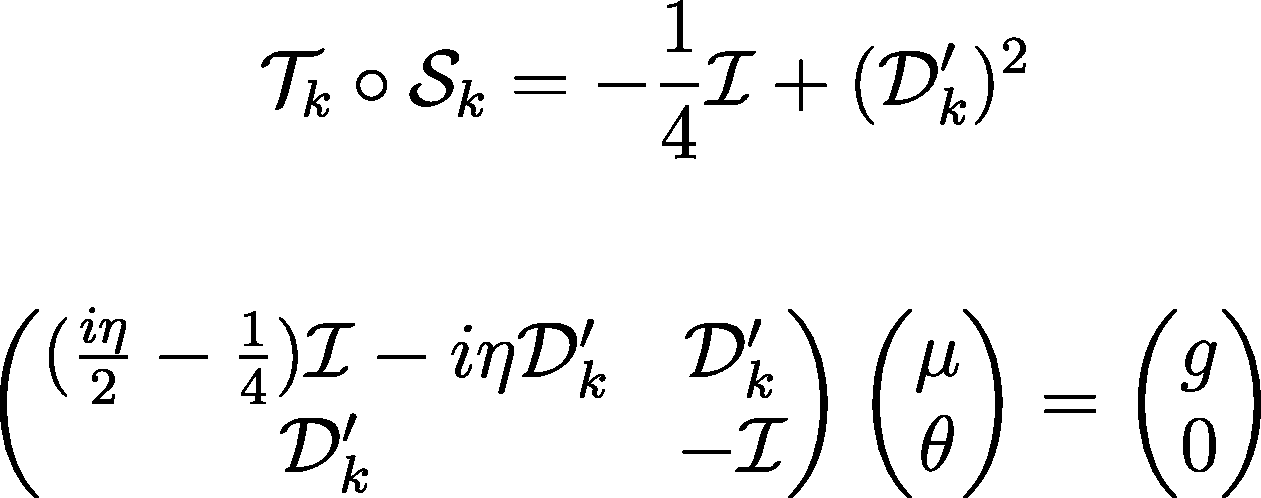
\includegraphics[width=0.6\textwidth]{assets/sound_hard_3.pdf}
\end{frame}


\begin{frame}

    \frametitle{Helmholtz - Sound Hard, Numerical Results I}

    \begin{columns}
        \begin{column}{0.5\textwidth}
            Experiment where density is generated by 50 random charged placed inside the torus.
        \end{column}
        \begin{column}{0.5\textwidth}
            \begin{figure}
                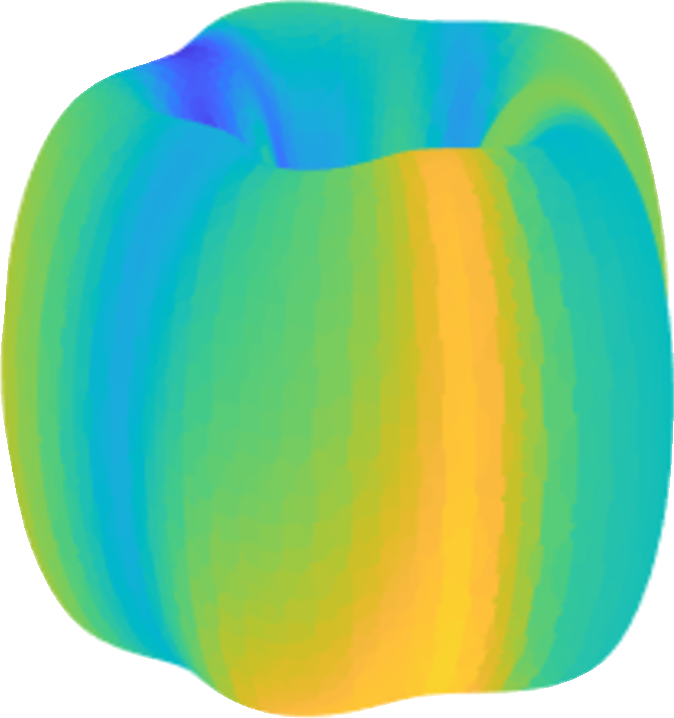
\includegraphics[width=0.6\textwidth]{assets/wiggly_torus_solved.pdf}
            \caption{Real component of density solved for $p=4$, $N_{\text{patch}} = 200$
                $N = 3000$.
            }
            \end{figure}
        \end{column}
    \end{columns}

\end{frame}

\begin{frame}
    \frametitle{Helmholtz - Sound Hard, Numerical Results II}

    \begin{figure}
        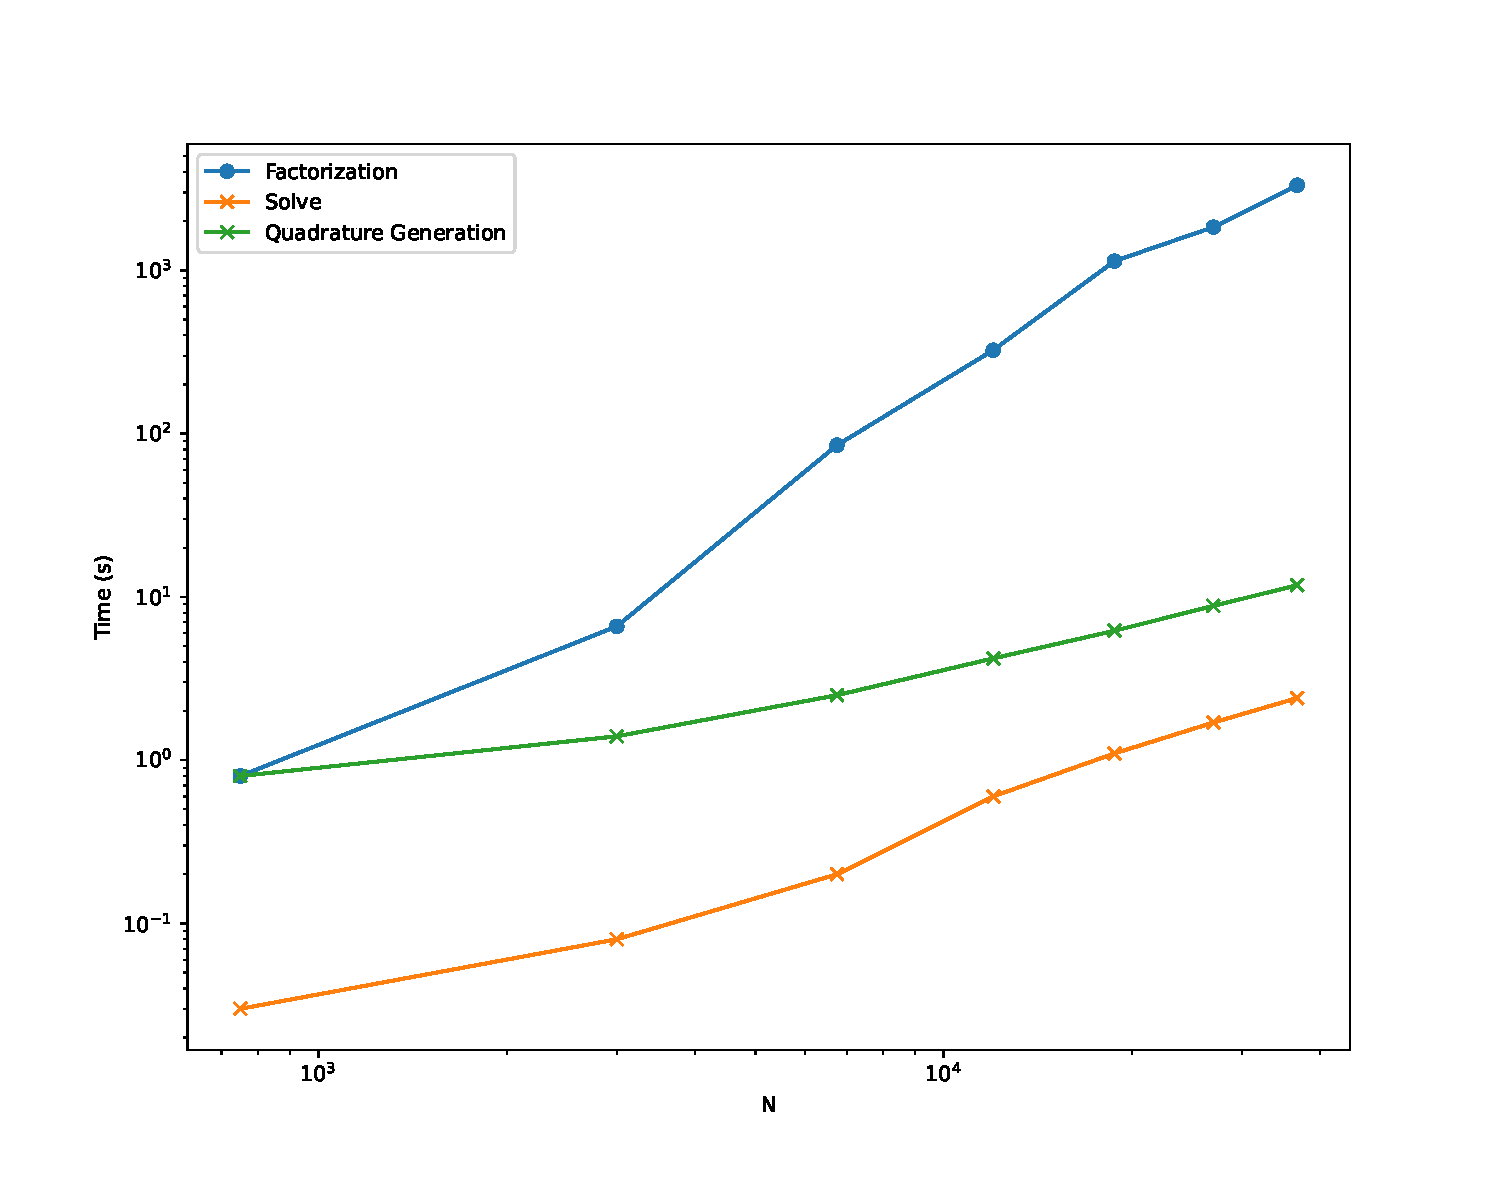
\includegraphics[width=\textwidth]{assets/scaling.pdf}
    \end{figure}
\end{frame}

\begin{frame}

    \frametitle{Helmholtz - Transmission}

\end{frame}


\begin{frame}

    \frametitle{Towards Maxwell}

    \centering
    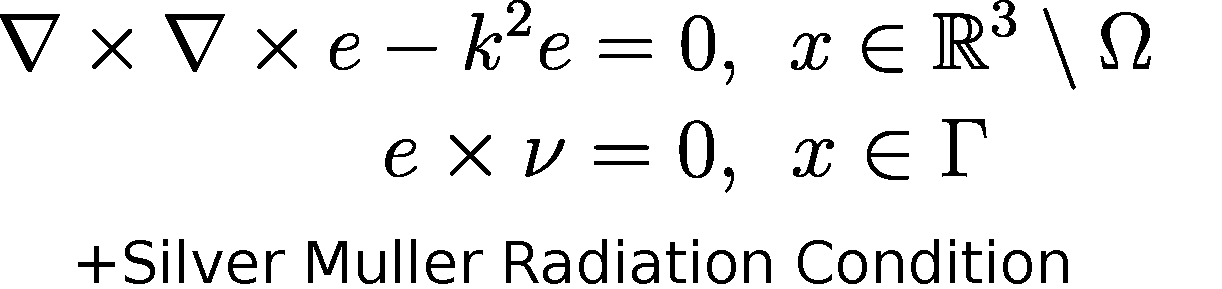
\includegraphics[width=0.6\textwidth]{assets/maxwell_scattering.pdf}

\end{frame}